\documentclass[a4paper, 12pt]{article}

\usepackage{hyperref}
\usepackage[warn]{mathtext}
\usepackage[utf8]{inputenc}
\usepackage[T2A]{fontenc}
\usepackage[english,russian]{babel}
\usepackage{multirow}
\usepackage{amsmath,amsfonts,amssymb,amsthm,mathtools}
\usepackage{indentfirst}
\DeclareSymbolFont{T2Aletters}{T2A}{cmr}{m}{it}
\usepackage{ gensymb }
\mathtoolsset{showonlyrefs=true}
\usepackage{euscript}
\usepackage{mathrsfs}
\usepackage[left=2cm,right=2cm,top=2cm,bottom=2cm]{geometry}
\usepackage{graphicx}
\usepackage{wrapfig}
\usepackage[rgb]{xcolor}
\hypersetup{
colorlinks=true,
urlcolor=blue
}


\title{Лабораторная работа}
\author{Гисич Арсений Б03-102}
\date{2022}

\begin{document}

	\begin{center}
		{\large МОСКОВСКИЙ ФИЗИКО-ТЕХНИЧЕСКИЙ ИНСТИТУТ (НАЦИОНАЛЬНЫЙ ИССЛЕДОВАТЕЛЬСКИЙ УНИВЕРСИТЕТ)}
	\end{center}
	\vspace{5 cm}
	{\Large
		\begin{center}
			{\bf Лабораторная работа 3.2.1}\\[0.2 cm]
			Сдвиг фаз в цепи переменнного тока
		\end{center}
	}
	\vspace{4 cm}
	\begin{flushright}
		{\Large Выполнил: \\
			\vspace{0.2 cm}
			Гисич Арсений \\
			\vspace{0.2 cm}
			Б03-109 \\}
	\end{flushright}
	\vspace{9 cm}
	\begin{center}
		Долгопрудный\\[0.1 cm]
		2022
	\end{center}
\thispagestyle{empty}

\section{Аннотация}

Целью данной работы является изучение влияние активного сопротивления, индуктивности и ёмкости на сдвиг фаз между током и напряжением в цепи переменного тока.

\section{Теоретические сведения}

Рассмотрим процессы, протекающие в контуре, подключённом к источнику внешней ЭДС, изменяющейся по грамоническому закону $\varepsilon = \varepsilon_0 \cos{(\omega t + \varphi_0)}$. Для напряжения на конденсаторе $U_C(t)$ получим уравнение 
\begin{equation}\label{eq1}
\ddot{U}_C + 2\gamma \dot{U}_C + \omega_0^2U_С = \varepsilon_0\cos{(\omega t + \varphi_0)}.
\end{equation}

Перейдём к комплексному представлению колебаний. Запишем уравнение~\eqref{eq1} в комплексной форме, обозначая комплексные величины как <<векторы>>:
\begin{align}\label{eq2}
U_C & = \mathtt{Re}\mathbf{U_C}, & \mathbf{U_C} & = \mathtt{Re}\mathbf{U_C} + i\mathtt{Im}\mathbf{U_C}, \\
\varepsilon & = \mathtt{Re}\mathbf{\varepsilon}, & \mathbf{\varepsilon} & = \mathbf{\varepsilon_0}e^{i\omega t} = \varepsilon_0e^{i(\omega t + \varphi_0)},
\end{align}
\begin{equation}\label{eq3}
\mathbf{\ddot{U}_C} + 2\gamma \mathbf{\dot{U}_C} + \omega_0^2\mathbf{U_С} = \omega_0^2\mathbf{\varepsilon}.
\end{equation}

Комплексный множитель $\mathbf{\varepsilon_0} = \varepsilon_0e^{i\varphi_0}$, стоящий перед $e^{i\omega t}$, называется \textit{комплексной амплитудой}.

Решив уравнение~\eqref{eq3}, получим комплескное выражение для напряжения на конденсаторе $\mathbf{U_C}$. \textit{Вещественная часть} этого решения $\mathtt{Re}\mathbf{U_C}$ и является решением исходного уравнения~\eqref{eq1}. Будем искать решение уравнения~\eqref{eq3} в виде
\begin{equation}\label{eq4}
\mathbf{U_C}(t) = \mathbf{U_{C0}}e^{i\omega t},
\end{equation}
где $\mathbf{U_{C0}}$ --- комплексная амплитуда напряжения на конденсаторе, не зависящая от времени. Подставляя \eqref{eq4} в \eqref{eq3}, находим $\mathbf{U_{C0}}$ и далее, комплексные амплитуды тока в контуре и напряжений на сопротивлении и индуктивности:
\begin{equation}\label{eq5}
\mathbf{U_{C0}} = \frac{\mathbf{\varepsilon_0}}{i\omega CZ}, \quad Z = R + i\left(\omega L - \frac{1}{\omega C}\right),
\end{equation}
\begin{equation}\label{eq6}
\mathbf{I_0} = \frac{\mathbf{\varepsilon_0}}{Z}, \quad \mathbf{U_{R0}} = \frac{R\mathbf{\varepsilon_0}}{Z}, \quad \mathbf{U_{L0}} = i\omega L\frac{\mathbf{\varepsilon_0}}{Z}.
\end{equation}

Комплексная величина $Z$ называется \textit{комплексным сопротивлением}, или \textit{импедансом}, последовательного контура. Можно определить импеданс каждого отдельного элемента контура:
\begin{equation}\label{eq7}
Z_R = R, \quad Z_L = i\omega L, \quad Z_C = \frac{1}{i\omega C}.
\end{equation}

В новых обозначениях уравнения \eqref{eq5}--\eqref{eq6} принимают вид
\begin{equation}\label{eq8}
\mathbf{I} = \frac{\mathbf{\varepsilon_0}}{Z}, \quad \mathbf{U_{R0}} = Z_R\mathbf{I_0}, \quad \mathbf{U_{C0}} = Z_C\mathbf{I_0}, \quad \mathbf{U_{L0}} = Z_L\mathbf{I_0}.
\end{equation}

Импеданс контура $Z$ не зависит от начальных условий, не содержит величин ни токов, ни напряжений, а определяется свойствами всех элементов, соединённых в контур, и частотой синусоидальной ЭДС, к которой он подклячён. Таким образом, \textit{импеданс $Z$ является характеристикой колебательного контура на заданной частоте}.

Выражение \eqref{eq5} для импеданса контура $Z$ содержит действительную часть $$\mathtt{Re}Z = R,$$ называемую \textit{активным} сопротивлением контура, и мнимую часть $$\mathtt{Im}Z = \omega L - \frac{1}{\omega C},$$ носящую название \textit{реактивного} сопротивления.

Импедансы контура и его отдельных элементов --- комплексные числа --- могут быть представленны в показательной форме:
\begin{equation}\label{eq9}
Z = Z_0e^{i\psi},
\end{equation}
где $Z_0 = |Z|$ --- модуль комплексного числа, $\psi = \mathtt{arg}Z$ --- его аргумент (фаза). Для импеданса рассматриваемого последовательного контура при этом находим
\begin{equation}\label{eq10}
Z_0 = \sqrt{(\mathtt{Re}Z)^2 + (\mathtt{Im}Z)^2} = \sqrt{R^2 + \left(\omega L - \frac{1}{\omega C}\right)^2} = \frac{R}{\cos{\psi_I}},
\end{equation}
\begin{equation}\label{eq11}
\tan{\psi_I} = \frac{\mathtt{Im}Z}{\mathtt{Re}Z} = \frac{\omega L - \frac{1}{\omega C}}{R}.
\end{equation}
Ток в контуре и напряжения на отдельных его элементах теперь могут быть получены по формулам~\eqref{eq5}--\eqref{eq8}. Например, действительная часть тока в контуре
\begin{equation}\label{eq12}
I(t) = \frac{\varepsilon_0}{R}\cos{\psi_I}\cos({\omega t + \varphi_0 - \psi_I)}.
\end{equation}
Как видно из~\eqref{eq11}~и~\eqref{eq12}, угол~$\psi_I$, определяемый отношением мнимой и действительной частей импеданса, представляют собой сдвиг фаз между напряжением на последовательном контуре и током в нём, причём \textit{положительные значения угла~$\psi_I$ соответствуют отставанию фазы тока, а отрицательные --- опережению}. В общем случае, когда к источнику последовательно подключены резистор, конденсатор и катушка самоиндукции, сдвиг фазы $\psi_I$ лежит в пределах $-\pi/2 < \psi_I < \pi/2$.

\section{Методика измерений}

Эталонная катушка $L$, магазин ёмкостей $C$ и магазин сопротивлений $R$ соединены последовательно и через дополнительное сопротивление $r$ подключены к источнику синусоидального напряжения --- звуковому генератору.

Сигнал, пропорцианальный току, снимается с сопротивления $r$, пропорциональный напряжению, --- с генератора. Оба сигнала подаются на осциллограф, имеющий два канала вертикального отклонения.

\section{Используемое оборудование}

\begin{enumerate}
    \item генератор звуковой частоты;
    \item двухканальный осциллограф;
    \item магазин ёмкостей;
    \item магазин сопротивлений;
    \item катушка индуктивности;
    \item резисторы;
    \item универсальный измеритель импеданса ($LCR$-метр);
\end{enumerate}

\section{Результаты измерений и обработка данных}

\subsection{RC-цепь}

Установленные параметры: $L = 50~мГн, \nu = 1~кГц$. Рассчитанное реактивное сопротивление цепи $$X_1 = 1/(\omega C) = 318~Ом.$$ Полученные значения сдвига фаз $\psi$ в зависимости от сопротивления $R$ представленны в таблице \ref{tab1}.

\begin{table}[h!]
\begin{center}
\begin{tabular}{|c|c|c|c|c|c|c|c|}
\hline
$R, Ом$   & $\sigma_R, Ом$ & $x_0, дел$ & $\sigma_{x_0}, дел$ & $x, дел$ & $\sigma_x, дел$ & $\psi, \pi \cdot рад$ & $\sigma_{\psi}, \pi \cdot рад$ \\ \hline
0,00    & 0,01   & 25,0    & 0,5      & -12,0  & 0,5     & -0,48       & -0,02        \\ \hline
300,00  & 0,01   & 25,0    & 0,5      & -6,5   & 0,5     & -0,26       & -0,02        \\ \hline
600,00  & 0,01   & 25,0    & 0,5      & -4,0   & 0,5     & -0,16       & -0,02        \\ \hline
900,00  & 0,01   & 25,0    & 0,5      & -2,5   & 0,5     & -0,10       & -0,02        \\ \hline
1800,00 & 0,01   & 25,0    & 0,5      & -1,0   & 0,5     & -0,04       & -0,02        \\ \hline
320,00  & 0,01   & 25,0    & 0,5      & -6,0   & 0,5     & -0,24       & -0,02        \\ \hline
240,00  & 0,01   & 25,0    & 0,5      & -7,0   & 0,5     & -0,28       & -0,02        \\ \hline
190,00  & 0,01   & 25,0    & 0,5      & -8,0   & 0,5     & -0,32       & -0,02        \\ \hline
\end{tabular}
\end{center}
\caption{RC-цепь}
\label{tab1}
\end{table}

Полученный график зависимости $ctg\,\psi = f(\omega CR_{\Sigma})$ представлен на рис.~\ref{ris1}.

\begin{figure}[h!]
\begin{flushleft}
    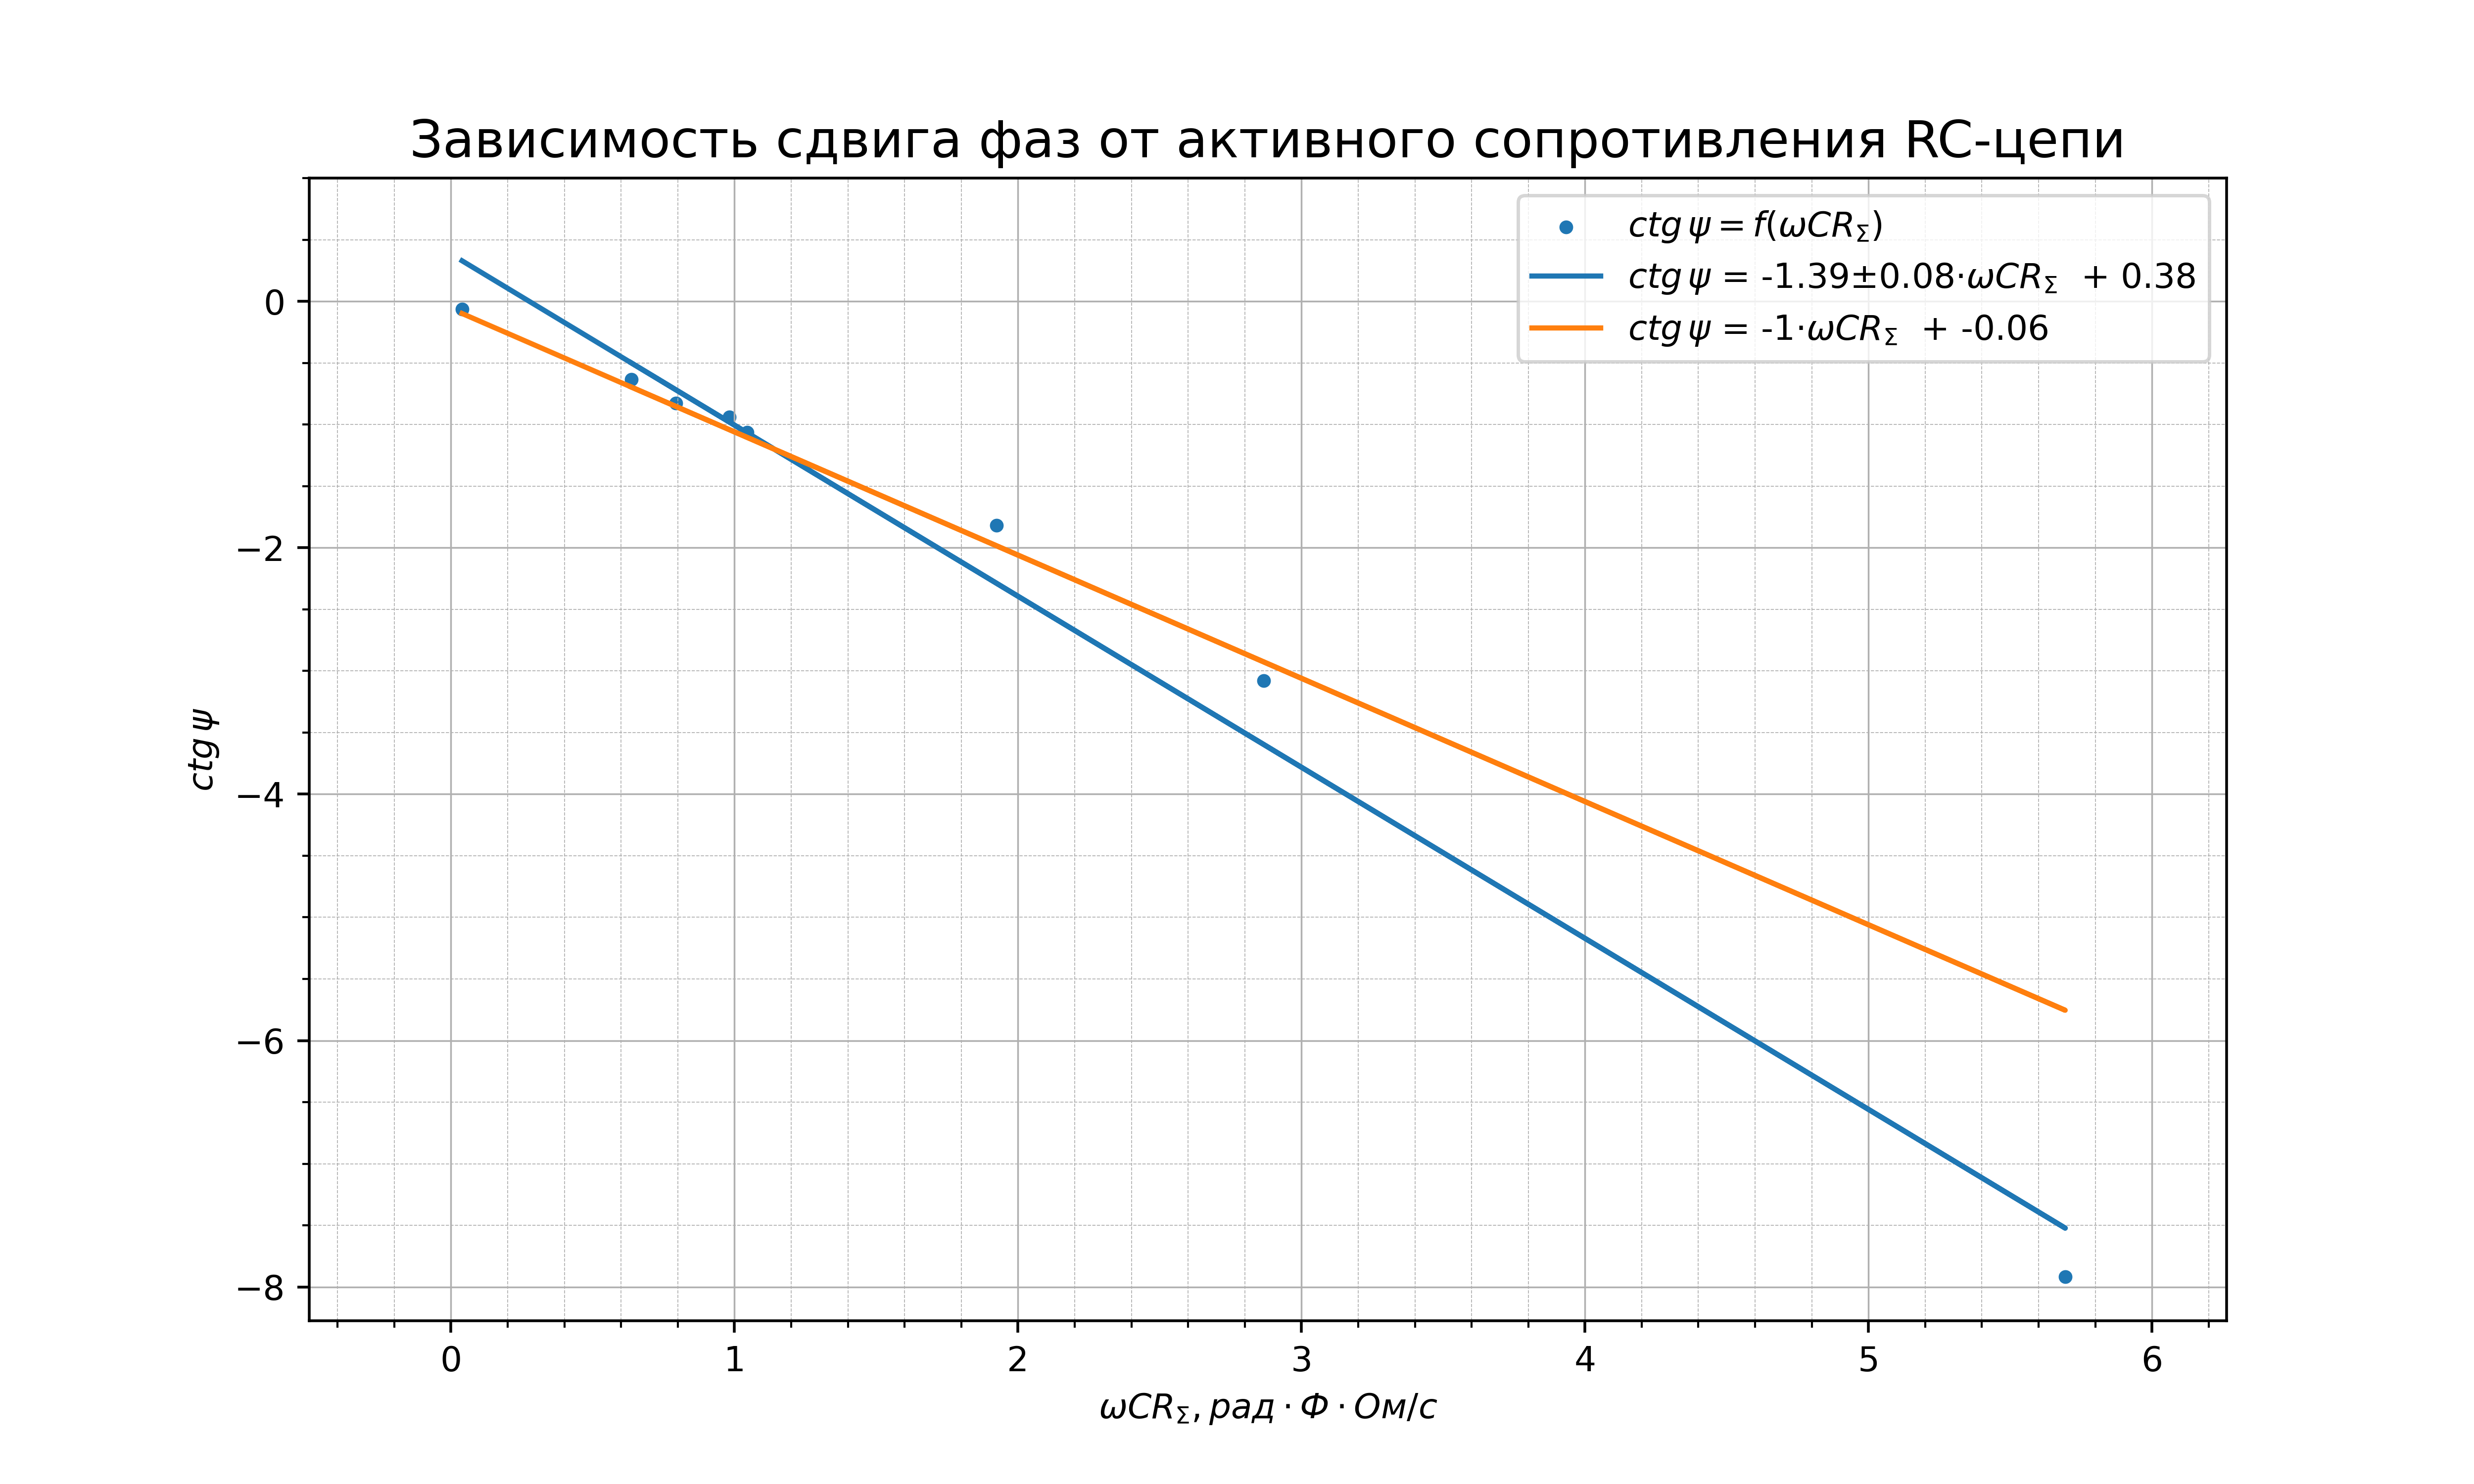
\includegraphics[scale=0.7]{3.2.1_1.png}
\end{flushleft}
\caption{}
\label{ris1}
\end{figure}

\section{Обсуждение результатов и выводы}

В данной работе исследовалась зависимость сопротивления проволоки от мощности выделяющегося на ней тепла. По результатам измерений для каждой температуры определялся коэффициент теплопроводности воздуха. Полученная зависимость представленна на рис. \ref{ris5}. Полученные значения для всех температур, кроме $70~\celsius$, согласуются с табличными данными -- $\kappa = 0,025\div0,030~Вт/(K \cdot м)$.
Использованный в работе метод измерений позволяет достичь относительной точности результатов в 20\%. Основной вклад в погрешность вносит погрешность определения коэффициентов линейной зависимости.

Также в данной работе был определён температурный коэффициент сопротивления молибдена:
$$\boxed{\alpha = \frac{1}{R_{273}}\frac{dR}{dT} = 0,0047\pm0,0008~K^{-1}}.$$
Табличное значение для данного коэффициента -- $0,0049~K^{-1}$, что согласуется с полученным результатом.

В простейшей модели твёрдых шариков коэффициент теплопроводности пропорционален корню абсолютной температруы $\kappa \varpropto T^{\frac{1}{2}}$. Эксперементальное значение показателя степени $$\boxed{\beta = 3,511\pm1,964},$$ что слабо согласуется с теорией. Во-первых, это может быть связано с неучтенными тепловыми потерями через основания цилиндра. Во-вторых, количество экспериментальных точек достаточно мало. В-третьих, при выводе формулы \eqref{3} пренебрегалось зависимостью теплопроводности от температуры, поэтому она справедлива только при $\Delta T \ll T$. И наконец, возникновение термо-ЭДС повлияло на точность вольтметра. Для получения более точного результата необходимо увеличить диапазон рабочих температур, количество экспериментальных точек и уменьшить шаг изменения температуры.

\end{document}